\section{Linear Programming}
\begin{itemize}
	\item Just like dynamic programming, there are different paradigms of programming, so for the following 
		lectures we'll explore linear programming.
\end{itemize}
\subsection{Example: Making Cake}
\begin{itemize}
	\item Suppose we're trying to make cake, and each item has a cost and associated profit. How much of 
		each item should we produce in order to maximize profit? 
	\item We're also given constraints, in terms of our supply of raw ingredients. 
	\item This falls under the category of \textit{constrained optimization}. They essentially ask us 
		to maximize a quantity, while satisfying certain constraints. We've actually done this before!
		\begin{itemize}
			\item When finding MSTs, the constraint was that our algorithm should have outputted some spanning
				tree. 
			\item For longest increasing subsequence, the constraint was that it was a subsequence and it is 
				an increasing one. 
		\end{itemize}
	\item The difference between these and linear programming is that the objective function (our goal)
		is a minimalization (or maximization) of a linear function of the decision variables. 
	\item Our goal is to find an algorithm that can solve all linear programs efficiently. 
\end{itemize}
\subsection{Decision Variables}
\begin{itemize}
	\item With decision variables we generally say that they are real values, and we \textbf{cannot} have 
		integer constraints in linear programs. If they do exist, then it's now called an Integer Linear 
		Programs (ILP), which has a completely different solution method.
	\item We now relax the constraints of \( x \) and \( y \) and allow them to take any value within 
		\( \mathbb R \)
\end{itemize}
\subsection{LP Standard Form}
\begin{itemize}
	\item A linear program in \textit{standard form} can be written as follows:

		We want to maximize the equation: \( c_1x_1 + c_2x_2 + \dots + c_n x_n \), subject to the constraints:
		\begin{align*}
			a_{11}x_1 + a_{12}x_2 + \dots + a_{1n}x_n &\le b_1\\
			a_{21}x_1 + a_{22}x_2 + \dots + a_{2n}x_n &\le b_2\\
													  & \vdots\\
			a_{m 1} x_1 + a_{m 2} x_2 + \dots + a_{mn}x_n &\le b_m
		\end{align*}
		and also $x_1, x_2, \dots x_n \ge 0$. In general, we say that we have $m$ constraints and $n$ variables 
		to satisfy. We can also write this in matrix form, where we want to maximize $\mathbf c^\top x$, 
		subject to the equations $A\mathbf x \le \mathbf b$ and $\mathbf x \ge 0$. Here, $\mathbf c$ and
		\( \mathbf c, \mathbf x \) are $1 \times n$ column vectors and $b$ is a $1 \times m$ column vector.

		\question{Why aren't we taking $c^\top x^\top$?}
\end{itemize}
\subsubsection{Classroom Allocation}
\begin{itemize}
	\item We have a set of courses and possible classrooms, and every course needs a classroom, but not 
		every course fits in every classroom! We want to find the maximum number of courses allocated 
		to a classroom.
	\item We can construct a graph $G = (V, E)$ where course $c$ can be assigned to classroom $r$ if and 
		only if $(c, r) \in E$. 
	\item We can make our decision variable \( x_{c, r} \)
		(ideally, boolean of 0 or 1, but this condition must be
		relaxed) for each pair $(c, r) \in E$. 
	\item Now for the constraints:
		\begin{itemize}
		\item Instead of constraining $x_{c, r}$ to 0 or 1, we can constrain $x_{c, r} \in [0, 1]$. As we'll 
			see, even though we've assumed $x_{c, r}$ can be real, they will turn out to be integers.
		\item We want the room to not be simultaneously assigned to more than one course (fully) at a time. So, 
			for all rooms $r$,
			\[
				\sum_{c:(c, r) \in E} x_{c, r} \le 1
			.\]
			In other words, for every room, the number of courses assigned to it must be less than 1. 
		\item We want every class to exist in one classroom only (so we don't have a situation 
			where half the class is in Wheeler and the rest is in Pimentel) , so for all classes $c$, 
			\[
				\sum_{r: (c, r) \in E} x_{c, r} \le 1
			.\]
			\question{Why isn't the constraint of $x_{c, r}\in [0, 1]$ sufficient to guarantee this condition?}

			\answer{Because there's multiple $x_{c, r}$ being assigned to \textit{every} pair! We want 
			the sum of all of these to be less than 1, so that part of the class isn't somewhere else.} 
		\end{itemize}
	\item Our objective is to find:
		\[
			\max \sum_{(c, r) \in E} x_{c, r}
		.\]
\end{itemize}
\subsection{Geometric Intuition}
\begin{itemize}
	\item Suppose we have the following LP when we're maximizing $x + 2y$ with the following constraints:
		\begin{align*}
			x &\le 3\\
			x + y &\le 5\\
			-3x + y &\le 1\\
			x \ge 0 & y \ge 0 
		\end{align*}
		We can graphically draw all of these constraints out, which will look as follows:
		\begin{center}
			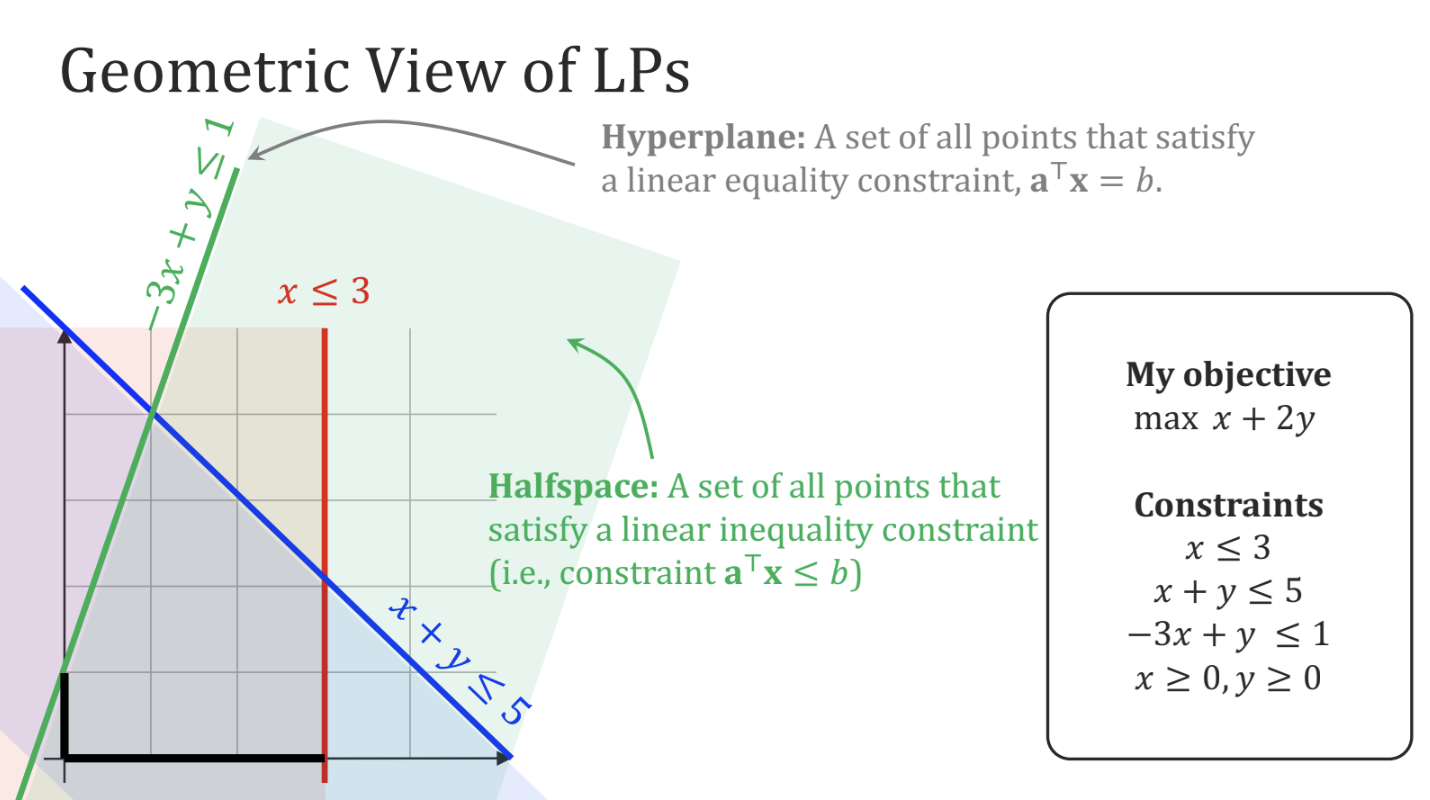
\includegraphics[scale=0.5]{LP-geo.png}
		\end{center}
		The overlap of these three regions defines the set where all our constraints are satisfied. We will 
		call this region the \textbf{feasible region}. This region is always going to be a \textbf{convex 
		region.}
	\item \textit{Definition:} A set $S$ is \textit{convex} if for any two points $x, y \in S$, all points 
		$z = \alpha x + (1 - \alpha) y$ for $\alpha \in [0, 1]$ satisfies $z \in S$.
		
		In other words, all points on the line connecting $x$ and $y$ are also in $S$. We can prove (proof 
		in slides) that every linear program will have a feasible set that is convex.
	\item Suppose now we're trying to maximize the equation $x + 2y$. To find the optimal solution, we have to 
		find \textit{level sets} of the feasible region, by considering $x + 2y = c$ and incrementing $c$.  
	\item \textit{Definition:} A vertex (or extreme point) is a point found at the intersection of 
		hyperplanes in \( \mathbb R \). 
	\item \textit{Claim:} Any linear program has an optimal solution that coincides with one of these vertices.
		Otherwise, the linear program could achieve unbounded values.  

		\question{So what exactly happens when one of the hyperplanes is parallel to our objective equation?}

		\answer{We can reasonably take any point on that face, but note that a corner will appear there too, 
			so there's no reason to not output the corner. In fact, almost all algorithms end up 
		finding corners anyway, since that's where the extreme points are guaranteed to exist.}  
\end{itemize}

\subsection{Algorithm for Finding Vertices}
\begin{itemize}
	\item Given $m$ constraints, for each subset of $n$ constraints, we find the intersection $x^*$ of these 
		constraints (do this by switching the inequalities with equalities and performing Gaussian elimination).
		If $x^*$ satisfies all constraints, then add it to the list of extreme points.  
	\item We could just go through all vertices and find the one with the highest payoff, but this would 
		be incredibly slow:
		\begin{itemize}
			\item There are \( m \choose n \) different vertices, and this number grows very quickly.   
			\item In fact, with $m = O(n)$ constraints, we can generate a situation where we have $2^n$ 
				different vertices: hypercubes!
		\end{itemize}
\end{itemize}
\subsection{Simplex}
\begin{itemize}
	\item  An algorithm that allows us to find the best neighboring vertex. Starting at $x^*$, look at all 
		neighbours of $x^*$. If $x^*$ is larger than all of these, return $x^*$. Otherwise, 
		move to the highest neighbour and repeat. 
	\item In higher dimensions, we define the neighbour is to say that two points are neighbours if they are 
		formed by swapping out a \textit{single} constraint. 
	\item Simplex is quite interesting, in the sense that in the worst case it does exactly what the naive 
		solution does, so its worst case runtime is still exponential. However, practically speaking, 
		Simplex is one of the fastest algorithms we know of!  

		It's even faster than some algorithms that provably run in polynomial time!   
\end{itemize}
